\chapter{HASIL YANG DIHARAPKAN}

\section{Hasil yang Diharapkan dari Penelitian}

% Ubah paragraf berikut sesuai dengan HASIL YANG DIHARAPKAN dari tugas akhir
Dari penelitian yang akan dilakukan, diharapkan pengendara yang sudah dilengkkapi alat dapat menentukan sebuah posisi 
mereka tanpa perlu mengkhawatirkan medan perlitasan yang dilewati (seperti \emph{underground and forest}) dengan 
penerapan metode \emph{Dead Reckoning} berbasis \emph{Deep Learning} sehingga menghasilkan luaran berupa navigasi 
secara \emph{Real Time} dengan akurasi tinggi.

\section{Hasil Pendahuluan}

% Ubah paragraf berikut sesuai dengan HASIL PENDAHULUAN dari tugas akhir
Sampai saat ini, penulis telah menyiapkan beberapa komponen alat, karena keterbatasan suku cadang maka penulis diharuskan 
\emph{Pre-Order} sensor MPU9255 hingga 28 hari dengan tujuan saat pengerjaan skripsi kedepannya hanya cukup pembuatan model dan dataset. 
Penulis juga sudah melakukan instalasi Mikrokontroller STM32 yang akan digunakan saat penelitian berlangsung, dan mencoba beberapa 
testing perhitungan jarak menggunakan \emph{Based Module Public} yang sudah ada di Github (https://github.com/topics/mpu9255), 
namun masih terdapat banyak error dan salah pemasangan yang sudah saya perbuat, karena itu memerlukan bimbingan lanjutan.

% Contoh input gambar dengan format *.jpg
\begin{figure} [ht] \centering
    % Nama dari file gambar yang diinputkan
    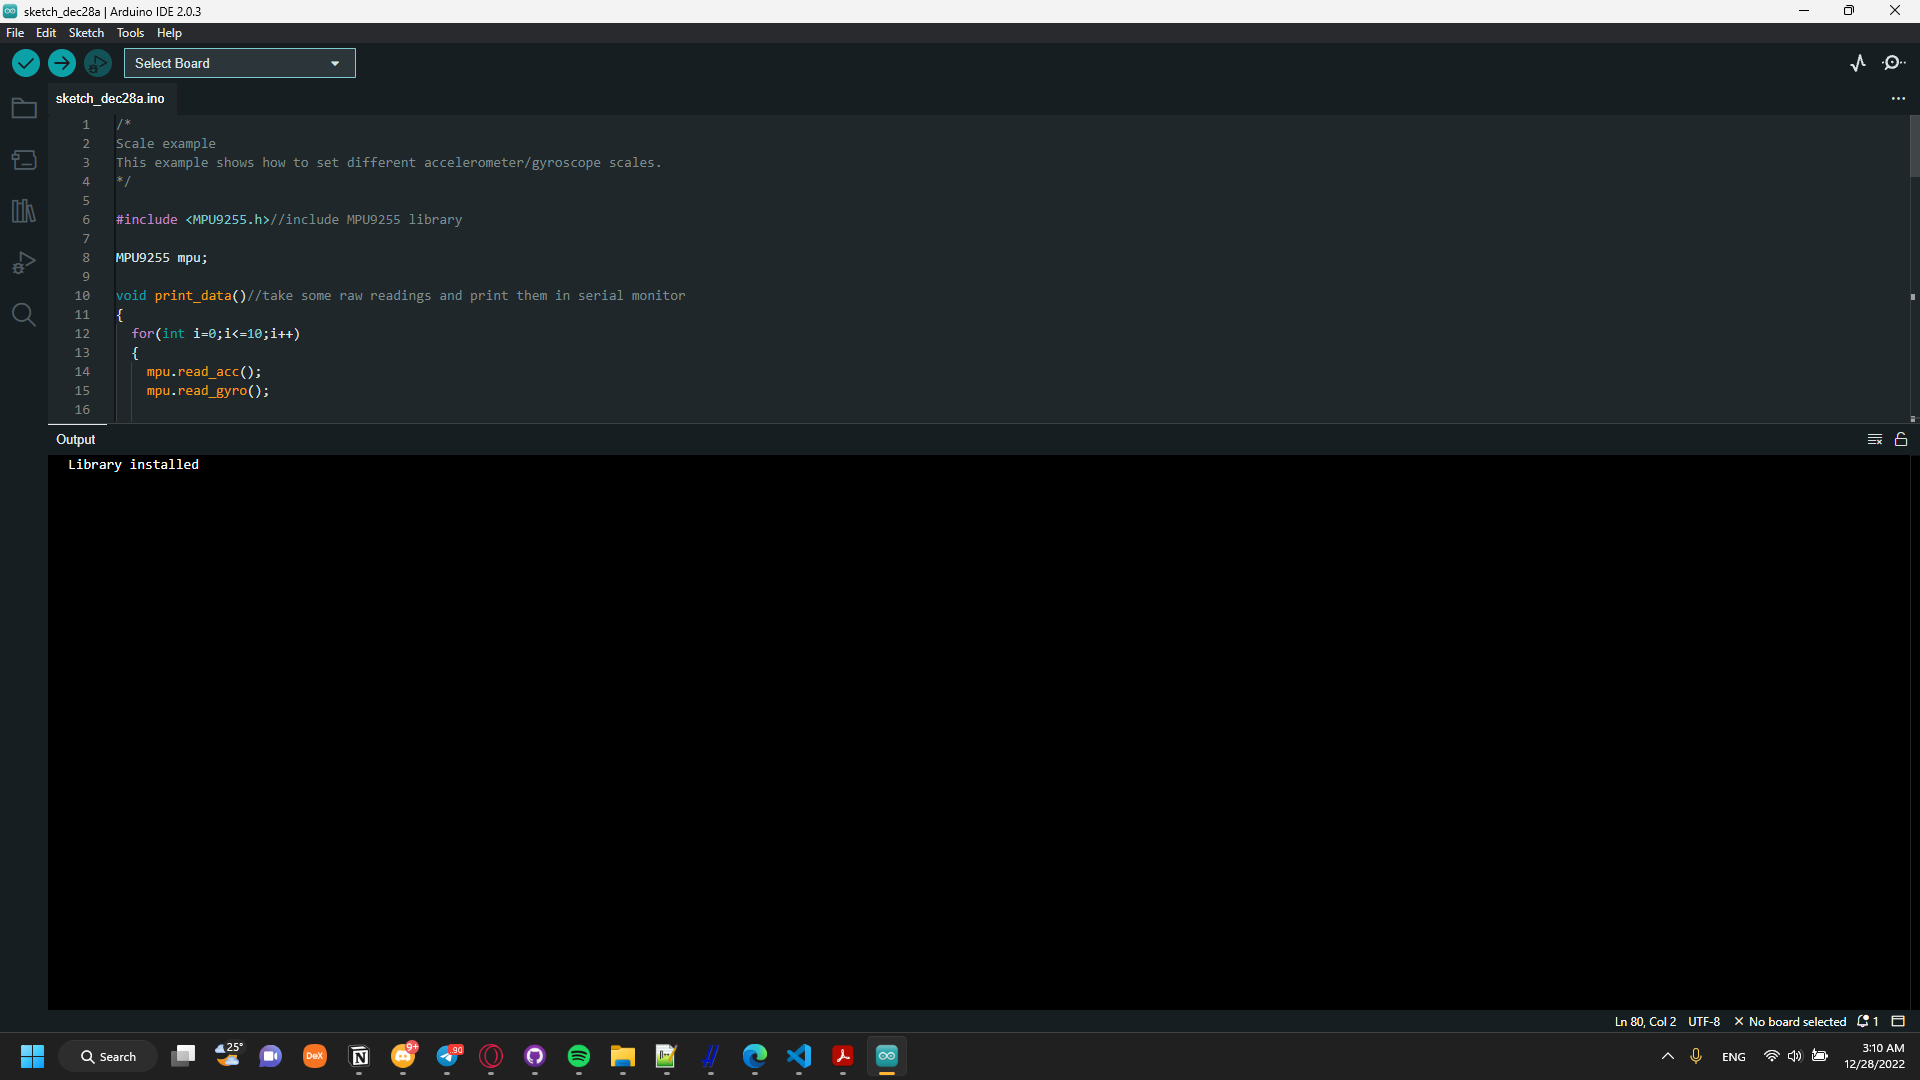
\includegraphics[scale=0.25]{gambar/Screenshot-2022-12-05.png}
    % Keterangan gambar yang diinputkan
    \caption{Screenshot pemasangan library MPU9255 di Arduino}
    % Label referensi dari gambar yang diinputkan
    \label{fig:lib-MPU9255}
  \end{figure}